%!TEX root = beamerCoursIsenLaTeX.tex
\documentclass[./beamerCoursIsenLaTeX.tex]{subfiles}

\begin{document}
%%%%%%%%%%%%%%%%%%%%%%%%%%%%%%%%%%%%%%%%%%%%%%%%%%%%%%%%%%%%%%%%%%%%%%%%%%%%%%
\section{Avoir de bonnes pratiques}
%%%%%%%%%%%%%%%%%%%%%%%%%%%%%%%%%%%%%%%%%%%%%%%%%%%%%%%%%%%%%%%%%%%%%%%%%%%%%%
\subsection{Organisation d'un dossier de cours}
%%%%%%%%%%%%%%%%%%%%%%%%%%%%%%%%%%%%%%%%%%%%%%%%%%%%%%%%%%%%%%%%%%%%%%%%%%%%%%
\begin{frame}
Un cours est divisé en : 
\begin{itemize}
\item Une présentation
\item[->] \emph{Qui se trouve dans le dossier "presentation"}
\item Des images
\item[->] \emph{Qui se trouve dans le dossier "images"}
\item Des TD
\item[->] \emph{Qui se trouve dans le dossier "TD"}
\item etc
\end{itemize}
\end{frame}
%%%%%%%%%%%%%%%%%%%%%%%%%%%%%%%%%%%%%%%%%%%%%%%%%%%%%%%%%%%%%%%%%%%%%%%%%%%%%%
\begin{frame}
\begin{figure}
\begin{center}
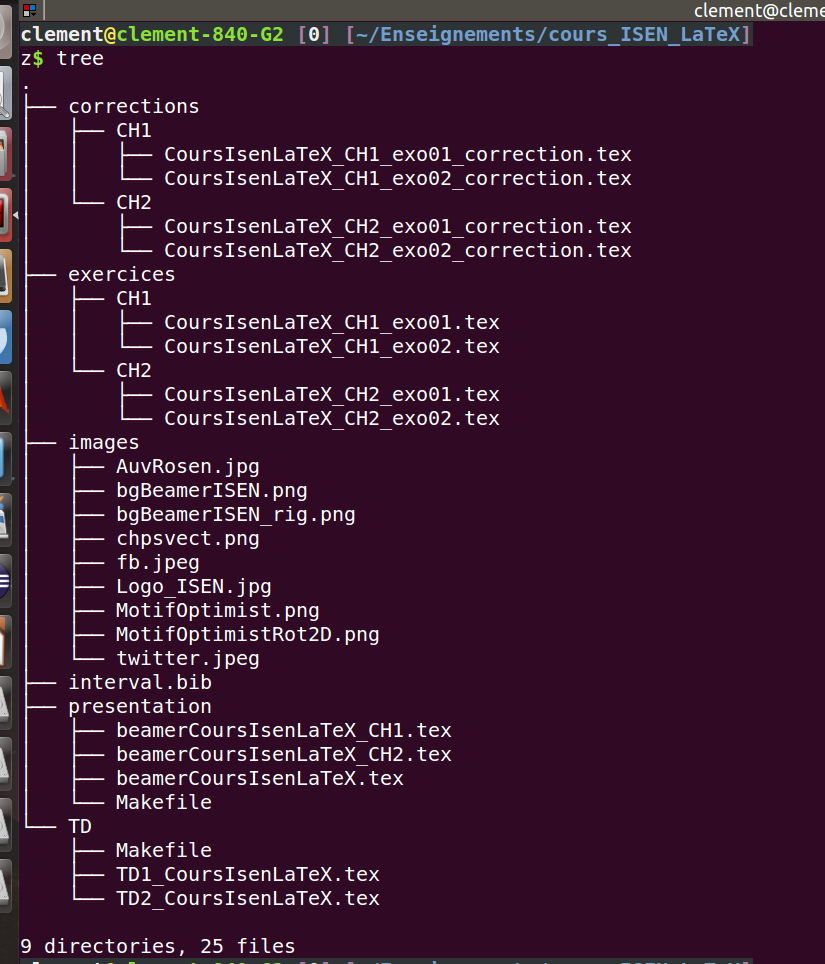
\includegraphics[height=0.7\textheight]{orgaCours.png}\label{fig::orgaCours}
\caption{organisation du cours.}
\end{center}
\end{figure}
\end{frame}
%%%%%%%%%%%%%%%%%%%%%%%%%%%%%%%%%%%%%%%%%%%%%%%%%%%%%%%%%%%%%%%%%%%%%%%%%%%%%%
\end{document}
